%%  Chapter 1 - Introduction
\ifpdf
\graphicspath{{chapters/Figs/}{chapters/Figs/Raster/}{Figs/PDF/}{Figs/}}
\else
\graphicspath{{chapters/Figs/}{chapters/Figs/Vector/}{Figs/}}
\fi

\chapter{Introduction}
\label{ch:introduction}

\section{The Indian Summer Monsoon and Synoptic Rainfall Variability}
\label{sec:intro_ism}

The Indian summer monsoon (ISM) is one of the most consequential
climate phenomena on Earth. Driven by the seasonal reversal of
atmospheric circulation between the cold Asian landmass and the warm
Indian Ocean, it delivers approximately 80\,\% of the Indian
subcontinent's annual precipitation over the four-month active season
from June to September \autocite{ding1994monsoon}. Nearly 1.4 billion
people depend on this rainfall for agriculture, freshwater
availability, and hydropower, making the ISM a pivotal determinant of
South Asian food security and economic output.

The ISM is characterized by pronounced spatial and temporal
variability, alternating widespread rainfall and break periods
of suppressed convection, operating across timescales from hours to
weeks to decades. A significant fraction of this variability at the
synoptic timescale of 3-10 days is organized by westward-propagating
disturbances collectively known as monsoon low-pressure systems (LPS).
Among these, Monsoon Depressions (MDs) represent the most dynamically
significant category: they are stronger than the more frequent monsoon
lows, yet weaker than tropical cyclones. Their slow northwestward
translation and broad precipitation shield (500-800\,km radius) make
them the largest contributors to heavy and sustained rainfall over
central and peninsular India.

The 2023 Cyclone Biparjoy, the 2021 low-pressure system over Odisha,
and the 2017 Bihar floods were all associated with systems that
maintained organised convection well beyond the expected 48-hour
post-landfall window. Each event produced multi-day flooding over the
Gangetic plain, affecting millions of people and causing agricultural
losses of billions of rupees. A reliable predictor of which
landfalling MDs will sustain inland, even a simple soil moisture
index computed at landfall time, would give district-level flood
forecast agencies an additional 48-72\,h of warning for evacuation
and pre-positioning of relief supplies.

%%  FIGURE: ERA5 JJAS mean rainfall over India (2001-2025)
\begin{figure}[H]
  \centering
  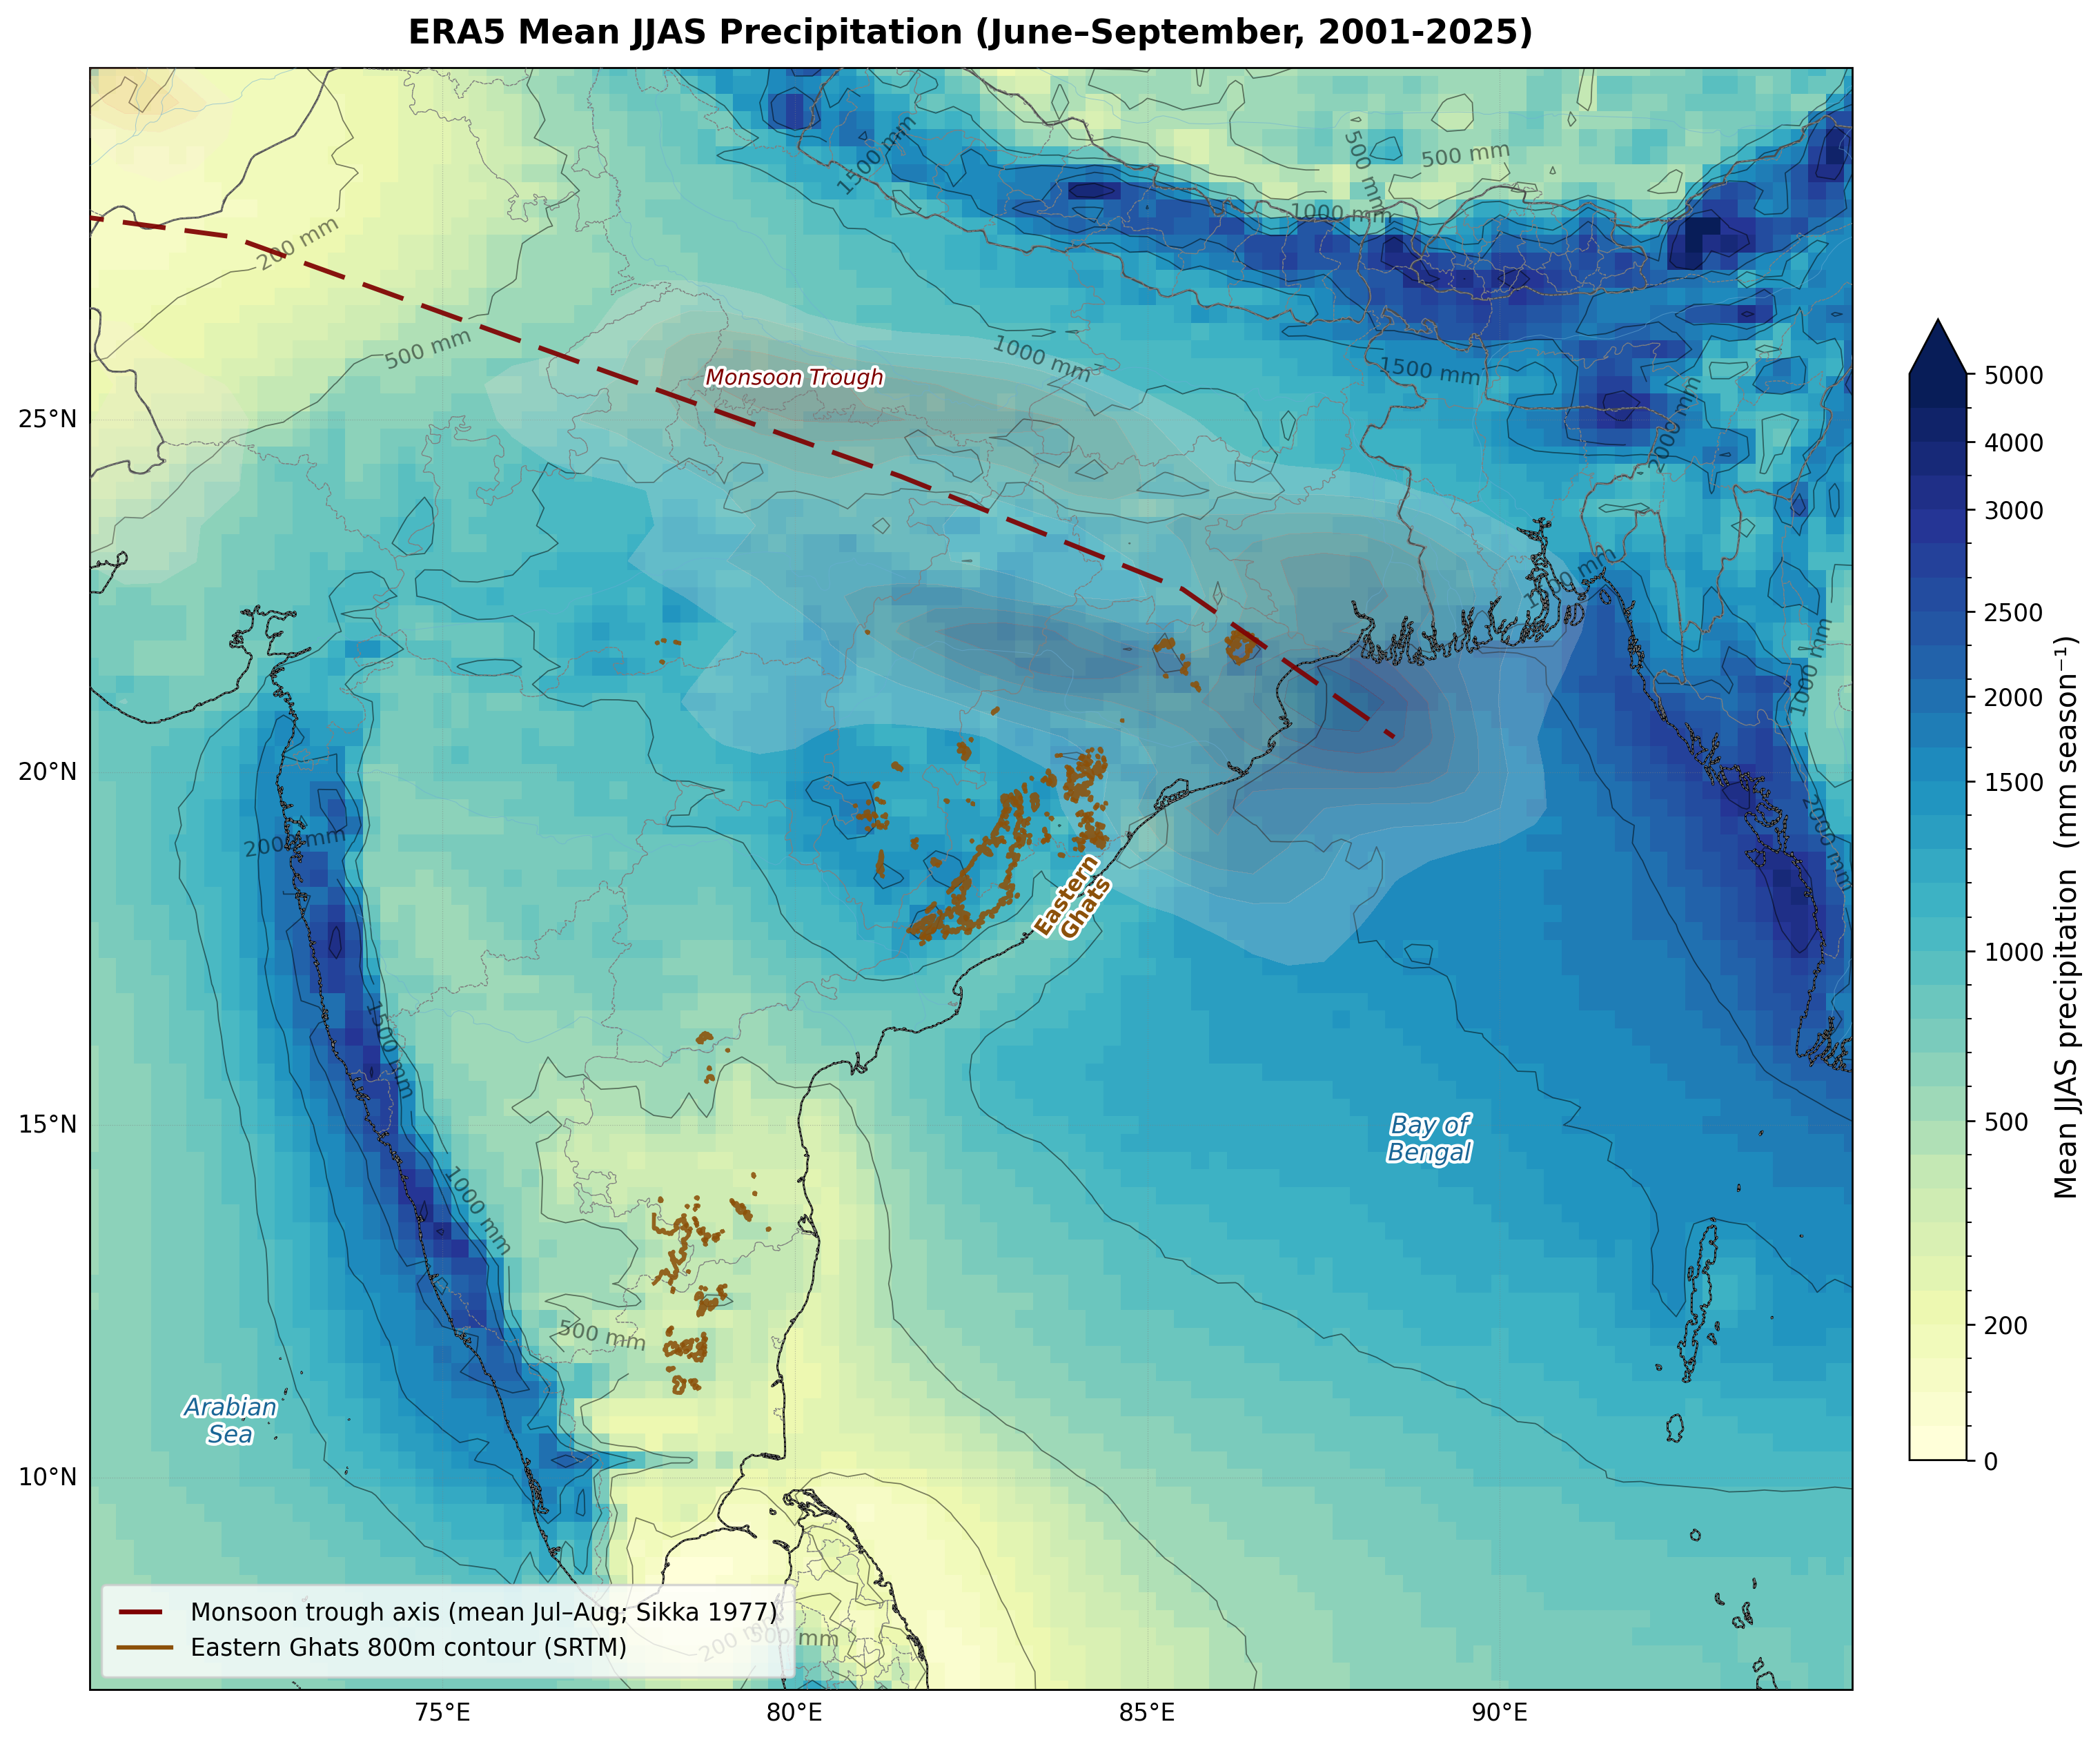
\includegraphics[width=0.9\textwidth]{india_jjas_climatology}
  \caption[JJAS seasonal rainfall climatology over India (2001-2025)]{Mean
  June-September precipitation (mm) over India from ERA5 (2001-2025).}
  \label{fig:india_rainfall_clim}
\end{figure}

% \section{Monsoon Depressions: Propagation, and the Post-Landfall Behavior}
\section{Monsoon Depressions \texorpdfstring{:}{} Propagation, and the Post-Landfall Behavior}
\label{sec:intro_md_problem}

Monsoon Depressions typically form over the Bay of Bengal (BoB)
during July and August, when warm sea-surface temperatures
(28-30$^\circ$C), deep atmospheric moisture, and strong low-level
cyclonic vorticity along the monsoon trough create favorable genesis
conditions. Historically, the BoB generates 5-6 MDs per year, with
substantial interannual variability tied to ENSO and Indian Ocean modes.

Before examining the post-landfall problem, it is useful to understand
two fundamental properties of these systems: why they rotate
anti-clockwise, and why they consistently track north-westward.

\subsection{Monsoon Depression Rotation}
\label{subsec:md_rotation}

All cyclonic weather systems in the Northern Hemisphere - including MDs -
rotate \emph{anti-clockwise} (cyclonically) as a direct consequence of the
\textbf{Coriolis force}. The Coriolis force is force arising from Earth's
rotation: in the Northern Hemisphere, any large-scale air parcel moving
toward a low-pressure center is deflected to its \emph{right}. This persistent
rightward deflection causes air flowing inward toward the low to curve
around it in a counter-clockwise sense, sustaining the cyclonic circulation
\autocite{holton2004introduction, sikka1977}. This is the same mechanism
responsible for the rotation of tropical cyclones, and even large eddies
in the ocean at sufficiently large scales.

In the case of an MD, the surface pressure minimum at the storm center
drives convergent inflow in the boundary layer. The Coriolis force
continuously deflects this inflow to the right, so that instead of
moving directly toward the center, air spirals cyclonically around it.
The Coriolis parameter $f = 2\Omega \sin\phi$ (where $\Omega$ is
Earth's angular velocity and $\phi$ is latitude) controls the strength
of this deflection: at the BoB and northern Indian latitudes
(10-25$^\circ$N), $f$ is large enough to enforce a well-organised
cyclonic vortex.

% Related images/webpages
% https://oceanservice.noaa.gov/education/tutorial_currents/04currents1.html
% https://www.weather.gov/source/zhu/ZHU_Training_Page/Miscellaneous/lowleveljet/lowleveljet.html
% Source for jet stream images:
% https://www.weather.gov/source/zhu/ZHU_Training_Page/Miscellaneous/lowleveljet/lowleveljet.html
\begin{figure}[H]
  \centering
  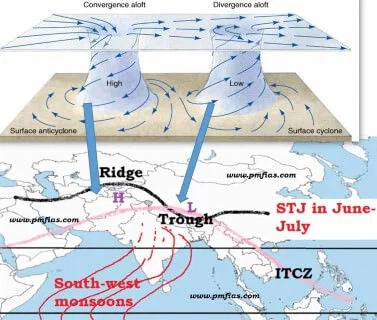
\includegraphics[width=0.75\textwidth]{Jet.png}
  \caption[Monsoon circulation]{The Sub-Tropical Westerly Jet (STJ)
    and its poleward retreat at monsoon onset, reducing vertical wind
    shear over the Bay of Bengal and
  permitting organised Monsoon Depression development.}
  \label{fig:Jet_stream_schematic_1}
\end{figure}

\subsection{Monsoon Depression North-Westward Propagation}
\label{subsec:md_propagation}

\begin{figure}[H]
  \centering
  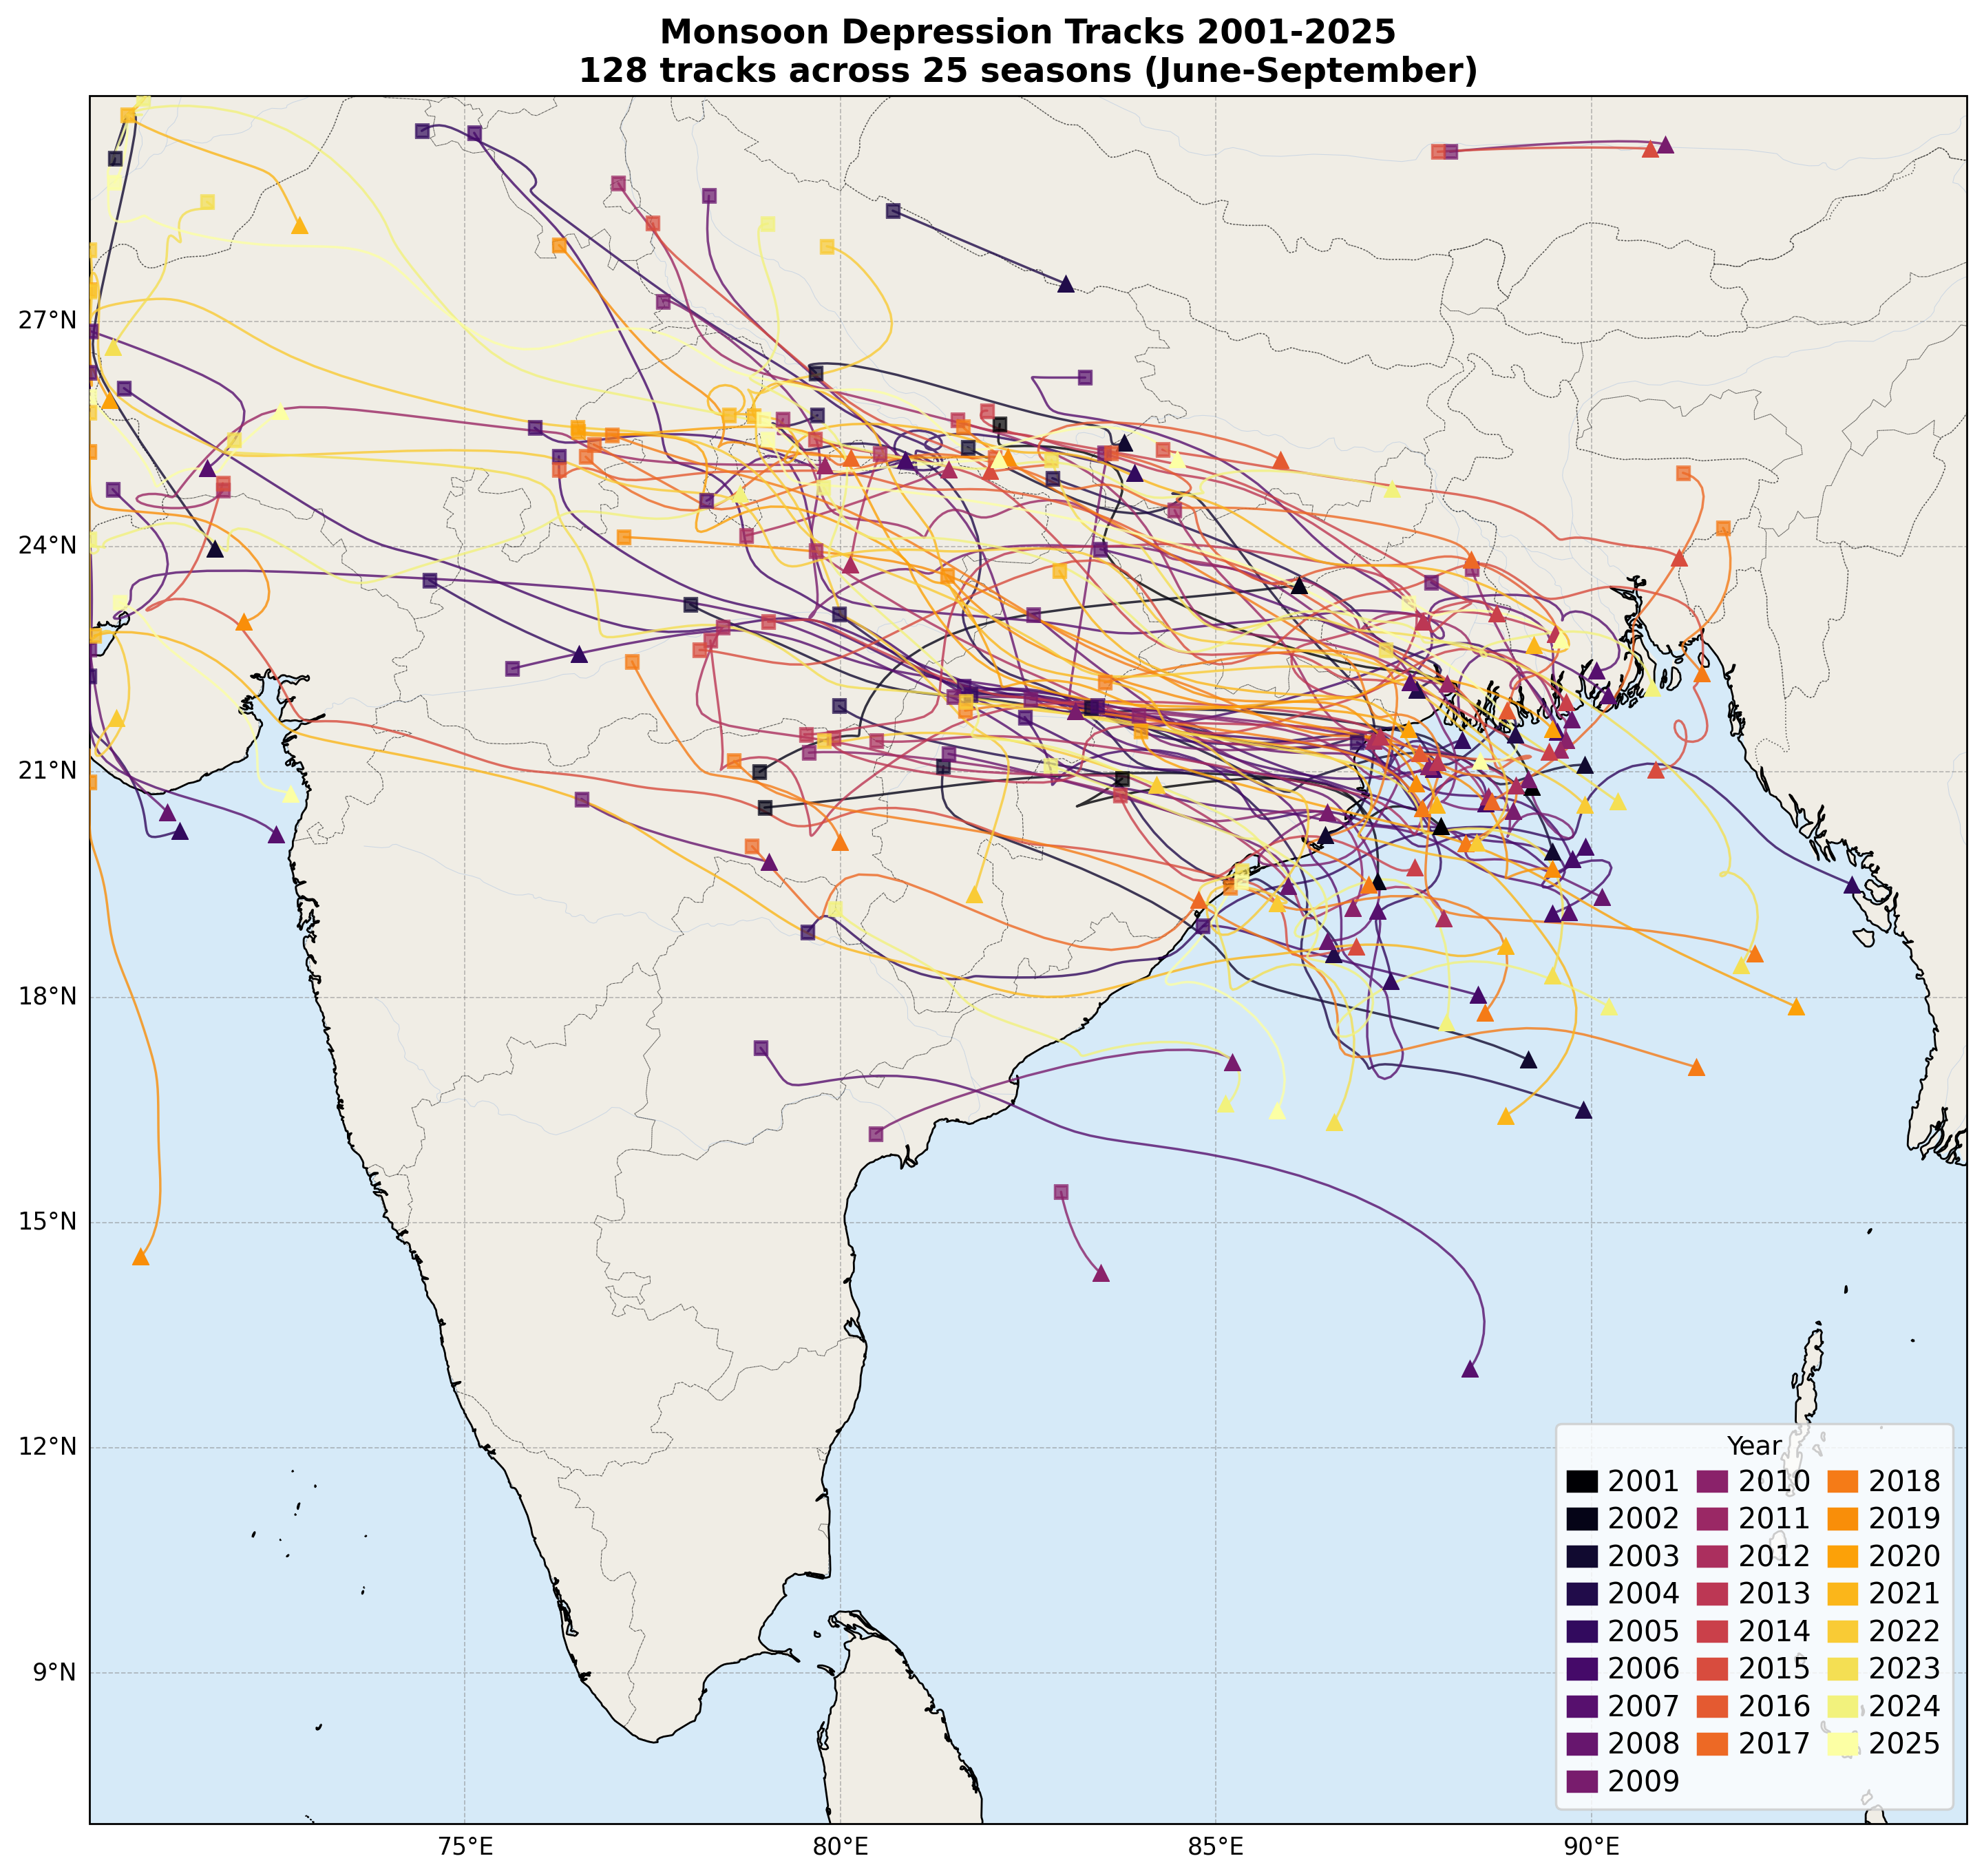
\includegraphics[width=0.9\textwidth]{all_years_tracks_map.png}
  \caption[Monsoon Propagation]{Monsoon depression detection from
  year 2001 to 2025}
  \label{fig:Monsoon_propagation}
\end{figure}

The characteristic north-westward translation of MDs results from the
following complementary mechanism operating on different scales

\begin{itemize}
  \item \textbf{Steering by the large-scale monsoon flow.} Once formed,
    an MD is steered predominantly by the mean environmental winds in
    the mid-troposphere (approximately the 500-700\,hPa layer). During
    the active ISM season, the large-scale monsoon circulation drives
    a mean westward and slightly northward flow across the BoB and
    northern India. The semi-permanent monsoon trough, extending from
    Pakistan across Rajasthan and central India to the BoB head,
    further guides the system along its north-westward axis
    \autocite{mishra2021monsoon, sikka1977}.
    % \item \textbf{The Somali Low-Level Jet and the Sub-Tropical Jet
    %   retreat.} The \textbf{Somali Low-Level Jet} (Findlater Jet), a
    %   powerful southwesterly stream at 850-925\,hPa
    %   \autocite{findlater1969}, intensifies during the active ISM and
    %   channels moisture from the Arabian Sea into the BoB. This jet
    %   also acts as a steering current, pushing disturbances
    %   north-westward into the Indian inland. At upper levels, the
    %   \textbf{Sub-Tropical Westerly Jet} retreats poleward of the
    %   Himalayas at monsoon onset \autocite{holton2004introduction},
    %   sharply reducing vertical wind shear over the BoB and permitting
    %   organised vortex development.
    % \item \textbf{Upper-level wind shear modulation.} At upper levels, the
    %   \textbf{Sub-Tropical Westerly Jet} (STJ) retreats poleward of the
    %   Himalayas at monsoon onset \autocite{holton2004introduction},
    %   sharply reducing vertical wind shear over the BoB and permitting
    %   organised vortex development.
\end{itemize}

The net effect of these steering mechanisms is a track directed
north-west (NW) or west-northwest (WNW) at translational speeds of
2-6\,m\,s$^{-1}$ (7-22\,km\,h$^{-1}$), making landfall preferentially
along the Odisha, West Bengal, and northern Andhra Pradesh coastlines.

Classical tropical meteorology theory predicts that a cyclonic system
should weaken rapidly upon crossing the coastline. Over the ocean,
the warm sea surface continuously restores latent and sensible heat
consumed by convection. As the system moves over land, this energy
source is removed. Surface friction simultaneously increases,
disrupting boundary-layer convergence and reducing the efficiency of
moisture transport into the inner core. Expected dissipation time is
24-48 hours after landfall - consistent with the decay observed in
most tropical cyclones.

In practice, a significant fraction of observed Indian MDs defies this
expectation. Cases in the 2001-2025 ERA5 detection record show systems
maintaining organised 850\,hPa vorticity and deep convection for 3-5
days and 800-1200\,km into the Indian inland. Understanding the physical
mechanisms enabling this persistence is a pressing operational
forecasting and climate impact problem.

% \section{The Brown Ocean Effect: Mechanism}
\section{The Brown Ocean Effect\texorpdfstring{:}{} Mechanism}
\label{sec:intro_boe}

\subsection{What is the Brown Ocean Effect?}
\label{subsec:boe_definition}

A compelling explanation for anomalous inland maintenance is the
\emph{Brown Ocean Effect} (BOE), first introduced and named by
\autocite{andersen2013}. The term ``Brown Ocean'' refers to the state
after a period of intense monsoon rainfall in which the saturated land
surface - visually brown and wet - mimics the energetic behaviour of a
warm tropical ocean. The BOE describes the process by which a
sufficiently wet land surface supplies \emph{latent heat flux} (LHF)
at rates comparable to a warm ocean, effectively replacing the oceanic
energy source after the MD makes landfall.

Over the ocean, sea-surface evaporation supplies latent heat to
sustain convection within the MD. When the storm crosses the coast,
it normally loses this energy supply. However, if the land surface
has been pre-moistened by antecedent monsoon rainfall to near field
capacity, the soil evaporates at the \emph{potential evaporation
rate} - the same rate as an ocean water surface - because water supply
is not limiting. The atmosphere above such a surface, the land
surface behaving thermodynamically like an ocean: high LHF, low Bowen
ratio (SHF/LHF), and a near-saturated boundary layer. This allows the MD's
convective organisation to persist for days after landfall.

\begin{figure}[H]
  \centering
  %% Right = ocean phase (evaporating blue ocean -> convection),
  %% Left = land phase (saturated brown soil -> comparable
  % evaporation -> convection),
  %% center = positive feedback loop arrow diagram)
  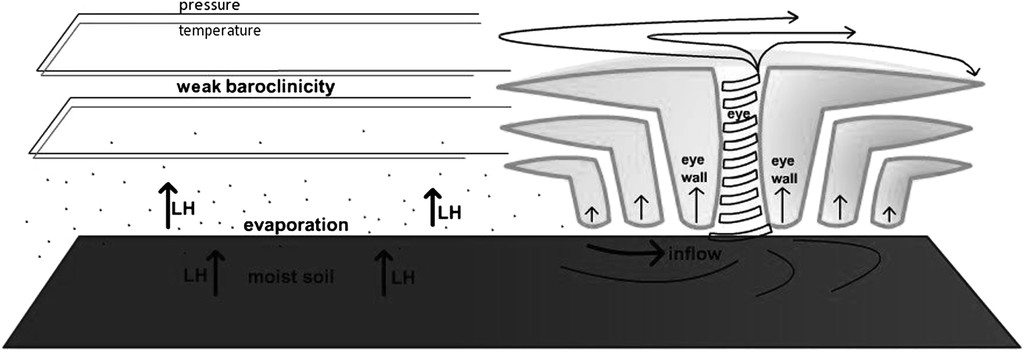
\includegraphics[width=0.8\textwidth]{BOE_schematic.jpg}
  \caption[Schematic of the Brown Ocean Effect mechanism]{The Brown
    Ocean Effect. Over pre-moistened land, saturated soil evaporates
    at the potential rate, sustaining LHF $\geq 70$\,W\,m$^{-2}$ and
  the precipitation-soil moisture feedback loop. Source: \autocite{andersen2013}.}
  \label{fig:boe_schematic}
\end{figure}

\subsection{The BOE Criterion}
\label{subsec:boe_criterion}

\cite{andersen2013} formalised the BOE with a measurable criterion:
\begin{equation}
  \text{LHF}_\text{inland} \geq 70\,\text{W\,m}^{-2}
  \quad \text{sustained for} \geq 18\,\text{consecutive hours after landfall.}
  \label{eq:boe_intro}
\end{equation}
This threshold of 70\,W\,m$^{-2}$ represents the minimum LHF that can
meaningfully sustain the moisture supply to deep convection within
the MD vortex. Systems meeting this criterion are termed \emph{BOE candidates}.

\subsection{Why the BOE Matters for Indian Monsoon Depressions}
\label{subsec:boe_significance}

The BOE is particularly significant in the Indian context for two reasons:
\begin{enumerate}
  \item \textbf{The BOE involves a self-reinforcing feedback loop.}
    The MD's own rainfall wets the soil beneath its track, which in
    turn sustains high LHF, which sustains subsequent convection and
    rainfall. This precipitation-soil moisture positive feedback
    (Figure~\ref{fig:boe_schematic}) means the BOE is not a passive
    response to antecedent conditions but an \emph{active} process
    that can maintain - and in some cases intensify - the surface
    energy supply during the land phase.
  \item \textbf{The land surface is pre-conditioned.} By July and
    August - peak MD months - the Gangetic plains and central India have
    received several weeks of monsoon rainfall, and near-surface soil
    moisture is frequently near field capacity. The land is ``charged''
    by antecedent rainfall before any MD arrives. This  \emph{antecedent
    soil moisture} effect - shown empirically by
    \autocite{kishtawal2013enhancement} to be predictor of inland penetration
    distance - is the critical enabling condition for the BOE over India.
\end{enumerate}

Without the BOE, post-landfall decay is controlled by surface
friction, reduced moisture flux, and the absence of oceanic thermal
forcing. With the BOE, the land surface functionally extends the
oceanic energy supply into the interior, explaining why certain MDs
persist for nearly a week and penetrate 1000-1200\,km inland.

The Eastern Ghats, however, introduce a complicating factor. This
discontinuous range of hills (600-1000\,m) along the eastern Deccan
margin intercepts the tracks of many landfalling MDs, slowing their
forward movement, enhancing windward precipitation, and potentially
disrupting the low-level moisture inflow that sustains inner-core
convection \autocite{houze1994}. Whether BOE-driven surface flux can
compensate for terrain-induced weakening and under what soil moisture
conditions is a key unresolved question motivating this thesis.

\section{Research Gap}
\label{sec:intro_gap}

Despite growing literature on the BOE in Atlantic and Gulf-coast
systems, and despite modelling and proxy evidence linking antecedent
soil moisture to Indian MD longevity \autocite{kishtawal2013enhancement,
osuri2020, hunt2017effect}, a systematic observational study of the
BOE in Indian MDs using storm-centerd diagnostics has not been
published. Previous Indian work relied on NWP experiments or
fixed-grid climatological correlations, without characterising the
azimuthal and radial evolution of LHF and soil moisture
\emph{relative to the moving storm center}. This storm-centerd
perspective is the primary methodological novelty of the present study.

\section{Research Objectives}
\label{sec:intro_objectives}

\begin{enumerate}
  \item Detect and characterise MD events from ERA5 over 2001-2025,
    validated against IMD reports, and classify them as short-lived
    ($<96$\,h) or long-lived ($\geq 96$\,h).
  \item Reconstruct the azimuthal and radial evolution of surface LHF,
    SHF, soil moisture (\texttt{SWVL1}), precipitation, and 2-m dew-point
    depression relative to the moving MD center via Azimuthal
    Hovm\"{o}ller analysis, comparing ocean and land phases.
    % \item Assess whether observed inland MDs satisfy the
    %   Andersen-Shepherd BOE criterion and document the landfall
    %   thermodynamic transitions distinguishing BOE candidates from
    %   conventionally decaying systems.
    % \item Quantify the role of antecedent soil moisture (exponentially
    %   weighted index over the future inland track corridor) in predicting
    %   inland penetration distance and post-landfall duration.
  \item Quantify the influence of antecedent soil moisture and
    terrain elevation. Characterise Eastern Ghats terrain influence
    on MD translational speed, precipitation asymmetry, and inland
    penetration using SRTM elevation data, and identify how this
    terrain interaction modulates the BOE.
\end{enumerate}

% \section{Thesis Organisation}
% \label{sec:intro_organisation}
%
% Chapter~\ref{ch:background} reviews tropical LPS energetics, MD
% structure and climatology, the BOE mechanism, land-atmosphere
% coupling, soil hydraulics, and Eastern Ghats orography.
% Chapter~\ref{ch:methodology} describes the ERA5 dataset, MD detection
% algorithm, Azimuthal Hovm\"{o}ller construction, time-series
% diagnostics, antecedent soil moisture index, heat flux analysis, and
% terrain characterisation.
% Chapter~\ref{ch:results} presents results in sequence: climatological
% overview $\rightarrow$ Hovm\"{o}ller diagnostics $\rightarrow$
% time-series thermodynamics $\rightarrow$ BOE classification
% $\rightarrow$ antecedent soil moisture $\rightarrow$ terrain interaction.
% Chapter~\ref{ch:discussion} synthesises these findings.
% Chapter~\ref{ch:conclusions} states the principal conclusions and
% future directions.
